% Gradient Info

\tikzset {_ahkgnj71m/.code = {\pgfsetadditionalshadetransform{ \pgftransformshift{\pgfpoint{262.5 bp } { 228 bp }  }  \pgftransformscale{3 }  }}}
\pgfdeclareradialshading{_bn94sccyc}{\pgfpoint{-88bp}{-56bp}}{rgb(0bp)=(0.96,0.96,0.96);
	rgb(0bp)=(0.96,0.96,0.96);
	rgb(5.25bp)=(0.86,0.86,0.89);
	rgb(12.25bp)=(0.72,0.73,0.78);
	rgb(20bp)=(0.87,0.87,0.89);
	rgb(25bp)=(0.96,0.96,0.96);
	rgb(400bp)=(0.96,0.96,0.96)}

% Gradient Info

\tikzset {_8s0cjt0cb/.code = {\pgfsetadditionalshadetransform{ \pgftransformshift{\pgfpoint{-69 bp } { 489 bp }  }  \pgftransformscale{3 }  }}}
\pgfdeclareradialshading{_arll6v0fl}{\pgfpoint{24bp}{-192bp}}{rgb(0bp)=(0.96,0.96,0.96);
	rgb(0bp)=(0.96,0.96,0.96);
	rgb(5.25bp)=(0.86,0.86,0.89);
	rgb(12.25bp)=(0.72,0.73,0.78);
	rgb(20bp)=(0.87,0.87,0.89);
	rgb(25bp)=(0.96,0.96,0.96);
	rgb(400bp)=(0.96,0.96,0.96)}

% Gradient Info

\tikzset {_xb2d8cp10/.code = {\pgfsetadditionalshadetransform{ \pgftransformshift{\pgfpoint{0 bp } { 0 bp }  }  \pgftransformrotate{0 }  \pgftransformscale{2 }  }}}
\pgfdeclarehorizontalshading{_9gf5dp3f7}{150bp}{rgb(0bp)=(0.6,0.85,1);
	rgb(37.5bp)=(0.6,0.85,1);
	rgb(62.5bp)=(0,0.5,0.5);
	rgb(100bp)=(0,0.5,0.5)}

% Gradient Info

\tikzset {_jwa1tz4np/.code = {\pgfsetadditionalshadetransform{ \pgftransformshift{\pgfpoint{0 bp } { 0 bp }  }  \pgftransformrotate{0 }  \pgftransformscale{2 }  }}}
\pgfdeclarehorizontalshading{_k1lfmkpnc}{150bp}{rgb(0bp)=(0.6,0.85,1);
	rgb(37.5bp)=(0.6,0.85,1);
	rgb(62.5bp)=(0,0.5,0.5);
	rgb(100bp)=(0,0.5,0.5)}

% Gradient Info

\tikzset {_lmp8db242/.code = {\pgfsetadditionalshadetransform{ \pgftransformshift{\pgfpoint{0 bp } { 0 bp }  }  \pgftransformscale{1 }  }}}
\pgfdeclareradialshading{_pt7yztjpq}{\pgfpoint{0bp}{0bp}}{rgb(0bp)=(1,1,1);
	rgb(0bp)=(1,1,1);
	rgb(25bp)=(0,0,0);
	rgb(400bp)=(0,0,0)}

% Gradient Info

\tikzset {_ksf0j3lzx/.code = {\pgfsetadditionalshadetransform{ \pgftransformshift{\pgfpoint{0 bp } { 0 bp }  }  \pgftransformscale{1 }  }}}
\pgfdeclareradialshading{_sd0lfnh1v}{\pgfpoint{0bp}{0bp}}{rgb(0bp)=(1,1,1);
	rgb(0bp)=(1,1,1);
	rgb(25bp)=(0,0,0);
	rgb(400bp)=(0,0,0)}

% Gradient Info

\tikzset {_sfydnlf8x/.code = {\pgfsetadditionalshadetransform{ \pgftransformshift{\pgfpoint{-246 bp } { -414 bp }  }  \pgftransformscale{2 }  }}}
\pgfdeclareradialshading{_xedxn5b0y}{\pgfpoint{136bp}{224bp}}{rgb(0bp)=(0.96,0.96,0.96);
	rgb(0bp)=(0.96,0.96,0.96);
	rgb(5.25bp)=(0.86,0.86,0.89);
	rgb(12.25bp)=(0.72,0.73,0.78);
	rgb(20bp)=(0.87,0.87,0.89);
	rgb(25bp)=(0.96,0.96,0.96);
	rgb(400bp)=(0.96,0.96,0.96)}
\tikzset{every picture/.style={line width=0.75pt}} %set default line width to 0.75pt   

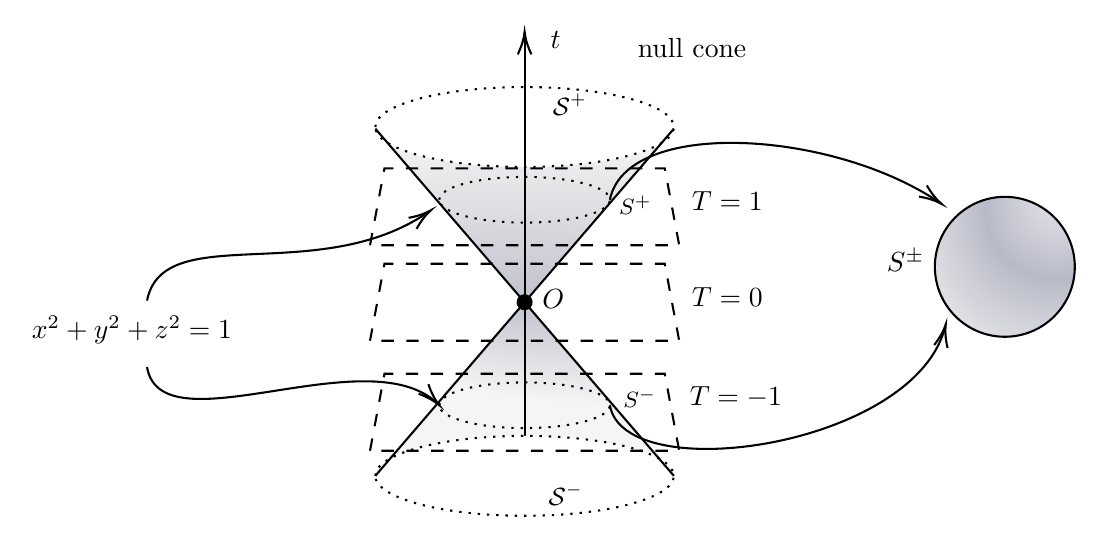
\begin{tikzpicture}[x=0.75pt,y=0.75pt,yscale=-1,xscale=1]
%uncomment if require: \path (0,240); %set diagram left start at 0, and has height of 240

%Shape: Triangle [id:dp9971590043766994] 
\draw  [draw opacity=0][shading=_bn94sccyc,_ahkgnj71m] (316.92,132.48) -- (388.83,216.92) -- (245,216.92) -- cycle ;
%Shape: Triangle [id:dp8161858650868445] 
\draw  [draw opacity=0][shading=_arll6v0fl,_8s0cjt0cb] (316.92,132.48) -- (388.83,48.85) -- (245,48.85) -- cycle ;
%Shape: Trapezoid [id:dp9657525832586118] 
\draw  [dash pattern={on 4.5pt off 4.5pt}] (242.44,151.83) -- (249.4,114.75) -- (384.44,114.75) -- (391.4,151.83) -- cycle ;
%Shape: Ellipse [id:dp6991681555350466] 
\draw  [fill={rgb, 255:red, 255; green, 255; blue, 255 }  ,fill opacity=1 ][dash pattern={on 0.84pt off 2.51pt}][line width=0.75]  (245,48.85) .. controls (245,38.22) and (277.2,29.6) .. (316.92,29.6) .. controls (356.64,29.6) and (388.83,38.22) .. (388.83,48.85) .. controls (388.83,59.49) and (356.64,68.1) .. (316.92,68.1) .. controls (277.2,68.1) and (245,59.49) .. (245,48.85) -- cycle ;
%Straight Lines [id:da6048999871668166] 
\draw    (316.92,49.67) -- (316.92,216.92) ;
%Straight Lines [id:da8004605643454383] 
\draw [shading=_9gf5dp3f7,_xb2d8cp10]   (316.92,133.29) -- (245,49.67) ;
%Straight Lines [id:da5641309946559745] 
\draw [shading=_k1lfmkpnc,_jwa1tz4np]   (316.92,133.29) -- (388.83,49.67) ;
\draw [shift={(316.92,133.29)}, rotate = 310.7] [color={rgb, 255:red, 0; green, 0; blue, 0 }  ][fill={rgb, 255:red, 0; green, 0; blue, 0 }  ][line width=0.75]      (0, 0) circle [x radius= 3.35, y radius= 3.35]   ;
%Shape: Ellipse [id:dp5518313431037392] 
\draw  [fill={rgb, 255:red, 255; green, 255; blue, 255 }  ,fill opacity=1 ][dash pattern={on 0.84pt off 2.51pt}] (245,216.92) .. controls (245,206.29) and (277.2,197.67) .. (316.92,197.67) .. controls (356.64,197.67) and (388.83,206.29) .. (388.83,216.92) .. controls (388.83,227.55) and (356.64,236.17) .. (316.92,236.17) .. controls (277.2,236.17) and (245,227.55) .. (245,216.92) -- cycle ;
%Straight Lines [id:da7941441583124655] 
\draw [shading=_pt7yztjpq,_lmp8db242]   (316.92,133.29) -- (245,216.92) ;
%Straight Lines [id:da3585204572517584] 
\draw [shading=_sd0lfnh1v,_ksf0j3lzx]   (316.92,133.29) -- (388.83,216.92) ;

%Straight Lines [id:da5552987525760773] 
\draw    (316.92,133.29) -- (316.92,4.92) ;
\draw [shift={(316.92,2.92)}, rotate = 90] [color={rgb, 255:red, 0; green, 0; blue, 0 }  ][line width=0.75]    (10.93,-3.29) .. controls (6.95,-1.4) and (3.31,-0.3) .. (0,0) .. controls (3.31,0.3) and (6.95,1.4) .. (10.93,3.29)   ;
%Shape: Trapezoid [id:dp11767877524393056] 
\draw  [dash pattern={on 4.5pt off 4.5pt}] (242.44,105.83) -- (249.4,68.75) -- (384.44,68.75) -- (391.4,105.83) -- cycle ;
%Shape: Ellipse [id:dp5991835638059029] 
\draw  [dash pattern={on 0.84pt off 2.51pt}] (275.82,83.92) .. controls (275.82,77.84) and (294.22,72.92) .. (316.92,72.92) .. controls (339.61,72.92) and (358.01,77.84) .. (358.01,83.92) .. controls (358.01,89.99) and (339.61,94.92) .. (316.92,94.92) .. controls (294.22,94.92) and (275.82,89.99) .. (275.82,83.92) -- cycle ;
%Shape: Trapezoid [id:dp03040677334653208] 
\draw  [dash pattern={on 4.5pt off 4.5pt}] (242.44,204.83) -- (249.4,167.75) -- (384.44,167.75) -- (391.4,204.83) -- cycle ;
%Shape: Ellipse [id:dp16350683172549307] 
\draw  [dash pattern={on 0.84pt off 2.51pt}] (275.82,182.92) .. controls (275.82,176.84) and (294.22,171.92) .. (316.92,171.92) .. controls (339.61,171.92) and (358.01,176.84) .. (358.01,182.92) .. controls (358.01,188.99) and (339.61,193.92) .. (316.92,193.92) .. controls (294.22,193.92) and (275.82,188.99) .. (275.82,182.92) -- cycle ;
%Curve Lines [id:da5556333810941549] 
\draw    (135,132.5) .. controls (142.75,93.31) and (217.32,126.24) .. (270.24,90.04) ;
\draw [shift={(271.83,88.92)}, rotate = 144.36] [color={rgb, 255:red, 0; green, 0; blue, 0 }  ][line width=0.75]    (10.93,-3.29) .. controls (6.95,-1.4) and (3.31,-0.3) .. (0,0) .. controls (3.31,0.3) and (6.95,1.4) .. (10.93,3.29)   ;
%Curve Lines [id:da7958034781622496] 
\draw    (135,164.5) .. controls (141.76,204.51) and (240.81,150.03) .. (274.81,181.92) ;
\draw [shift={(275.82,182.92)}, rotate = 225.86] [color={rgb, 255:red, 0; green, 0; blue, 0 }  ][line width=0.75]    (10.93,-3.29) .. controls (6.95,-1.4) and (3.31,-0.3) .. (0,0) .. controls (3.31,0.3) and (6.95,1.4) .. (10.93,3.29)   ;
%Shape: Circle [id:dp0994570688091998] 
\path  [shading=_xedxn5b0y,_sfydnlf8x] (514.58,116.21) .. controls (514.58,97.59) and (529.68,82.5) .. (548.29,82.5) .. controls (566.91,82.5) and (582,97.59) .. (582,116.21) .. controls (582,134.82) and (566.91,149.92) .. (548.29,149.92) .. controls (529.68,149.92) and (514.58,134.82) .. (514.58,116.21) -- cycle ; % for fading 
\draw   (514.58,116.21) .. controls (514.58,97.59) and (529.68,82.5) .. (548.29,82.5) .. controls (566.91,82.5) and (582,97.59) .. (582,116.21) .. controls (582,134.82) and (566.91,149.92) .. (548.29,149.92) .. controls (529.68,149.92) and (514.58,134.82) .. (514.58,116.21) -- cycle ; % for border 

%Curve Lines [id:da472614963631488] 
\draw    (358.01,83.92) .. controls (365.77,44.73) and (463.84,49.81) .. (516.26,84.85) ;
\draw [shift={(517.83,85.92)}, rotate = 214.7] [color={rgb, 255:red, 0; green, 0; blue, 0 }  ][line width=0.75]    (10.93,-3.29) .. controls (6.95,-1.4) and (3.31,-0.3) .. (0,0) .. controls (3.31,0.3) and (6.95,1.4) .. (10.93,3.29)   ;
%Curve Lines [id:da301798245305416] 
\draw    (358.01,182.92) .. controls (364.78,222.93) and (504.01,203.32) .. (519.4,145.68) ;
\draw [shift={(519.83,143.92)}, rotate = 102.43] [color={rgb, 255:red, 0; green, 0; blue, 0 }  ][line width=0.75]    (10.93,-3.29) .. controls (6.95,-1.4) and (3.31,-0.3) .. (0,0) .. controls (3.31,0.3) and (6.95,1.4) .. (10.93,3.29)   ;


% Text Node
\draw (328,1.5) node [anchor=north west][inner sep=0.75pt]    {$t$};
% Text Node
\draw (396,78.5) node [anchor=north west][inner sep=0.75pt]    {$T=1$};
% Text Node
\draw (396,124.5) node [anchor=north west][inner sep=0.75pt]    {$T=0$};
% Text Node
\draw (395,172.5) node [anchor=north west][inner sep=0.75pt]    {$T=-1$};
% Text Node
\draw (78,138.5) node [anchor=north west][inner sep=0.75pt]    {$x^{2} +y^{2} +z^{2} =1$};
% Text Node
\draw (324,125.5) node [anchor=north west][inner sep=0.75pt]    {$O$};
% Text Node
\draw (370,4.5) node [anchor=north west][inner sep=0.75pt]   [align=left] {null cone};
% Text Node
\draw (361,80.5) node [anchor=north west][inner sep=0.75pt]  [font=\footnotesize]  {$S^{+}$};
% Text Node
\draw (363,173.5) node [anchor=north west][inner sep=0.75pt]  [font=\footnotesize]  {$S^{-}$};
% Text Node
\draw (329,31.5) node [anchor=north west][inner sep=0.75pt]  [font=\small]  {$\mathcal{S}^{+}$};
% Text Node
\draw (327,219.5) node [anchor=north west][inner sep=0.75pt]  [font=\small]  {$\mathcal{S}^{-}$};
% Text Node
\draw (490,106.5) node [anchor=north west][inner sep=0.75pt]    {$S^{\pm }$};

\end{tikzpicture}